\chapter{Метод обучения с подкреплением} \label{chapt1}
При постановке задач обучения с подкреплением (Reinforcement learning, коротко RL) исследуемую систему условно разделяют на два блока: агент и динамический процесс или среда. Агент - структурно автономная система, которая в процессе функционирования системы производит наблюдения, выбирает действие и применяет это действие на среду, меняя её состояние. Схематичная визуализация взаимодействия показана на рисунке \ref{img:rl} Цель агента - выбирать адекватные задаче действия.

\begin{figure}[ht] 
	\center
	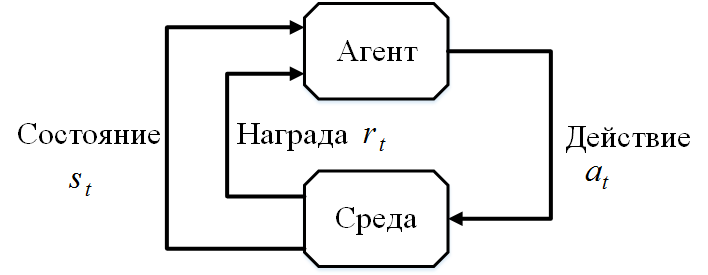
\includegraphics [scale=0.7] {rl}
	\caption{Схема взаимодействия агента со средой} 
	\label{img:rl}  
\end{figure}

В процессе обучения агент принимает специальный скалярный сигнал от среды - подкрепление. Этот сигнал показывает, насколько хорошо агент выполняет поставленную задачу. Обычно этот сигнал связывается только с теми событиями, которые кардинально влияют на процесс: успешное выполнение части задачи, задачи целиком (сигнал награды) или же наоборот, критическая ошибка агента (сигнал штрафа), приведшая к драматическим событиям. Именно этот аспект отличает обучение с подкреплением от обучения с учителем (supervised learning), при котором предоставляются пары <<входные данные - ответ>>. 

\section{Постановка задачи управления с применением обучения с подкреплением} \label{sect1_1}

В произвольный момент времени $ t_i $ агент принимает состояние среды $ s_i\in S $, где $ S $ некоторое конечное множество возможных состояний внешней среды, и, базируясь на этой информации, вырабатывает определенное воздействие на среду $ a_i\in A(s_i) $, где $ A(s_i) $ конечное множество действий, которые могут быть оказаны на среду в состоянии $ s_i $. Данное воздействие $ a_i $ переводит среду в состояние $ s_{i+1} $, а агент получает вознаграждение $ r_i $. Агент в процессе обучения должен выработать такую стратегию $ \pi: S \rightarrow A $, чтобы максимизировать $ R_i $ - суммарную величину всех подкреплений.

Различают два типа задач обучения с подкреплением:
\begin{itemize}
	\item задачи с терминальным состоянием - эпизодические;
	\item задачи без терминального состояния - непрерывные.
\end{itemize}

Для эпизодической задачи $ R_i $ определяется как:
\begin{equation}
\label{eq:1_1p1}
\begin{alignedat}{2}
R_i=r_{i+1} + r_{i+2} + \cdots + r_N = \sum \limits_{k=i}^{N}r_{i+1+k} \end{alignedat}
\end{equation}
где $ i $ - номер шага, а $ N $ - количество шагов в эпизоде.

В отличии от эпизодических задач, где эпизод состоит из конечного числа шагов и суммарная величина подкрепления всегда может быть ограничена некоторой максимальной величиной, непрерывные задачи могут иметь $ R_i $ стремящееся к бесконечности. Для таких случаев применяют выражение:
Для эпизодической задачи $ R_i $ определяется как:
\begin{equation}
\label{eq:1_1p2}
\begin{alignedat}{2}
R_i=r_{i+1} + \gamma \cdot r_{i+2} + \gamma^2 \cdot r_{i+3} + \cdots = \sum \limits_{k=0}^{\infty}\gamma^k \cdot r_{i+1+k}
\end{alignedat}
\end{equation}
где $ \gamma \in [0, 1]$ - коэффициент дисконтирования подкрепления, который обеспечивает сходимость суммарной величины подкрепления.  
Параметр дисконтирования взвешивает значения подкрепления, полученные в прошлом относительно новых. Чем ближе $ \gamma $ к единице, тем больше агентом принимаются во внимание новые сигналы от среды, а если $ \gamma = 0 $, то все будущие сигналы подкрепления никак не будут учтены. 
%\newpage\S
%============================================================================================================================

\section{Использование знаний и исследование среды} \label{sect1_2}
Как уже было сказано, целью функционирования агента является максимизация суммарного подкрепления, что достигается выбором наиболее подходящих воздействий. В процессе обучения агент вырабатывает случайные воздействия и анализирует полученные подкрепления. Однако, через некоторое время после начала обучения агент уже обладает некоторыми знаниями о среде и может их использовать для достижения цели функционирования. Агент должен уметь находить компромис между процессами использования данных и исследования среды. Существуют две основные стратегии нахождения баланса между этими процессами:

\begin{itemize}
	\item <<жадная>> стратегия;
	\item <<$ \epsilon $-жадная>> стратегия.
\end{itemize}

<<Жадная>> стратегия предполагает выбор агентом воздействий в соответствии с накопленными знаниями. В случае полных знаний агента о среде выбираемые воздействия будут наилучшими. 

При <<$ \epsilon $-жадной>> стратегии определяется параметр $ \epsilon \in [0; 1] $, с вероятностью $ \epsilon $ агент исследует среду, то есть выбирает случайное воздействие, и с вероятностью $ 1-\epsilon $ агент выбирает воздействие в соответствии с накопленными знаниями - <<жадное>> воздействие.

При старте обучения, в условиях отсутствия знаний о среде, предпочтительна <<$ \epsilon $-жадная>> стратегия с $ \epsilon > 0.5$. В процессе исследования среды и накопления знаний рекомендуется постепенно снижать $ \epsilon $ до 0, когда $ \epsilon = 0 $ стратегия становится <<жадной>>.

\section{Функции оценки} \label{sect1_3}
Как уже было показано, обучение с подкреплением имеет дело с наградами и штрафами, которые принимаются от среды, но данные сигналы имеют сиюминутный характер и не могут прямо использоваться как данные о качестве работы агента. Практически все алгоритмы обучения с подкреплением используют функции оценки, которые бывают двух видов:
\begin{itemize}
	\item функция оценки состояния среды (value function);
	\item функция оценки воздействия агента на среду (Q-function).
\end{itemize}

Функция оценки состояния среды обозначается как $ V $ и связывает состояние среды $ s $ c её оценкой $ V(s) $. Для стратегии управления $ \pi $ оценка состояния среды $ s $ будет определятся как сумма всех подкреплений, которые получит агент в будущем следуя данной стратегии управлений:
 
$$ V^\pi(s)=R_i=\sum \limits_{k=0}^{\infty}\gamma^k \cdot r_{i+1+k}. $$

\noindent где $ s $ - состояние среды на текущем шаге($ s_i=s $), $ i $ - текущий шаг. 

$ V^\pi(s) $ можно выразить через оценку состояния среды и сигнал подкрепления на следующем шаге:

\begin{equation}
\label{eq:1_2p1}
\begin{alignedat}{2}
V^\pi(s)=r_{i+1} + \gamma\cdot\sum\limits_{k=0}^{\infty}\gamma^k \cdot r_{i+2+k}=r_{i+1} + \gamma \cdot V^\pi(s_{i+1}).
\end{alignedat}
\end{equation}

Функция оценки воздействия обозначается $ Q $ и связывает состояние среды $ s $ и воздействие $ a $ с оценкой воздействия $ Q(s,a) $. Для стратегии управления $ \pi $ оценка воздействия $ a $ при состоянии среды $ s $ определяется как сумма будущих подкреплений начиная с состояния $ s $ и если агент применит воздействие $ a $:

\begin{equation}
\label{eq:1_2p2}
\begin{alignedat}{2}
Q^\pi (s,a) = R_i = \sum\limits_{k=0}^{\infty}\gamma^k \cdot r_{i+1+k}.
\end{alignedat}
\end{equation}

\noindent где $ a $ - воздействие на шаге $ i $ ($ a=a_i $). Предполагается, что действие $ a $ на следующем шаге и далее будет удовлетворять стратегии $ \pi $, то есть $ a_k=\pi(s_k) $ для всех $ k=i+1, i+2, i+3, ... $ Оценка воздействия на текущем шаге выражается через оценку воздействия на следующем шаге и подкрепление на следующем шаге:

\begin{equation}
\label{eq:1_2p3}
\begin{alignedat}{2}
Q^\pi (s,a) = r_{i+1} + \gamma\cdot\sum\limits_{k=0}^{\infty}\gamma^k \cdot r_{i+2+k}=r_{i+1} + \gamma \cdot Q^\pi(s_{i+1}, \pi(s_{i+1})).
\end{alignedat}
\end{equation}

Функцию оценки состояния среды можно выразить через функцию оценки воздействия, зная при этом стратегию управления. Для этого необходимо для каждого состояния определить воздействие исходя из стратегии управления $ a_i = \pi(s_i) $:

\begin{equation}
\label{eq:1_2p4}
\begin{alignedat}{2}
V^\pi(s) = Q^\pi(s, \pi(s)).
\end{alignedat}
\end{equation}

Подставляя (\ref{eq:1_2p4}) в (\ref{eq:1_2p3}) получив формулу нахождения оценки воздействия на текущем шаге через оценку состояния на следующем:

\begin{equation}
\label{eq:1_2p5}
\begin{alignedat}{2}
Q^\pi(s, a) = r_{i+1} + \gamma\cdot V^\pi(s_{i+1}).
\end{alignedat}
\end{equation}

\section{Оптимальная стратегия управления} \label{sect1_4}

От стратегии управления агента зависят функция оценки состояния среды и функция оценки воздействия. Допустим, стратегия управления $ \pi $ лучше, чем стратегия $ \pi '$, так как при стратегии $ \pi $ суммарная величина всех подкреплений больше, чем при $ \pi '$. То есть можно говорить о том, что стратегия $ \pi $ лучше или равна $ \pi '$ потому что $ V^{\pi} \geq V^{\pi '} $ при $ s \in S $. Таким образом, существует по крайней мере одна стратегия управления, лучше или эквивалента всем другим стратегиям управления и такая стратегия называется оптимальной. Оптимальная стратегия может быть не одна, все оптимальные стратегии обозначаются $ \pi^* $. 

Для поиска оптимальной стратегии существуют различные методы:
\begin{itemize}
	\item генетические алгоритмы - поиск лучшей стратегии из случайных;
	\item градиентный спуск - поиск определенных параметров стратегии;
	\item динамическое программирование.
\end{itemize}
На практике обычно используются комбинации этих методов, которые дают наиболее эффективный алгоритм управления.


\section{Уравнение Беллмана и оптимальные функции оценки} \label{sect1_5}

Оптимальные стратегии управления $ \pi^* $ используют функцию состояния среды $ V^* $, которую называют оптимальной функцией состояния среды: 

\begin{equation}
\label{eq:1_5p1}
\begin{alignedat}{2}
V^*(s) = \smash{\displaystyle\max_{\pi}} \: V^{\pi}(s),
\end{alignedat}
\end{equation}

\noindent для всех $ s \in S $.

Также, все оптимальные стратегии управления $ \pi^* $ используют одинаковую функцию оценки воздействия, которая называется оптимальной функцией воздействия и обозначается $ Q^* $:

\begin{equation}
\label{eq:1_5p2}
\begin{alignedat}{2}
Q^*(s, a) = \smash{\displaystyle\max_{\pi}} \: Q^{\pi}(s, a),
\end{alignedat}
\end{equation}

\noindent для всех $ s \in S $ и $ a \in A $.
 
Для нахождения оптимальных функций оценки воздействия и состояния среды необходимо определить рекуррентные формулы. В соответствии с формулой (\ref{eq:1_2p5}) оптимальная функция оценки воздействия $ Q^* $ для каждой пары $ (s, a) $ определяет размер подкрепления в зависимости от выбранного действия $ a $ при состоянии среды $ s $ и суммарную величину подкрепления на следующем шаге при условии следования оптимальной стратегии $ \pi^* $:

\begin{equation}
\label{eq:1_5p3}
\begin{alignedat}{2}
Q^*(s, a) = r_{i+1} + \gamma\cdot V^*(s_{i+1}),
\end{alignedat}
\end{equation}

\noindent где $ i $ - текущий шаг, $ s_i=s, a_i=a $.

В соответствии с (\ref{eq:1_2p1}) и (\ref{eq:1_5p1}) определим оптимальную функцию оценки состояния $ s $:  

\begin{equation}
\label{eq:1_5p4}
\begin{alignedat}{2}
V^*(s) = \smash{\displaystyle\max_{a \in A(s)}} \: (r(s, a) + \gamma \cdot V^*(f(s, a))),
\end{alignedat}
\end{equation}

\noindent где $ r(s, a) $ - функция, определяющая размер подкрепления, полученного от среды при состоянии $ s $ при выборе воздействия $ a $; $ f(s, a) $ - функция, определяющая новое состояние внешней среды при текущем состоянии $ s $ и при выборе агентом воздействия $ a $. Уравнение 
\ref{eq:1_5p4} называют уравнением Беллмана []. Из этого уравнения может быть найдена оптимальная функция оценки состояния, однако для этого необходимо будет решать систему уравнений из $ N_s $ уравнений для каждого состояния внешней среды $ s_k \in S, k=\overline{1,N_s} $, где $ N_s $ количество элементов в множестве $ S $ при известных функциях $ r(s, a) $ и $ f(s, a) $, описывающих динамику среды. Сложность нахождения оптимальной функции оценки состояния среды данным образом заключается в том что функции $ r(s, a) $ и $ f(s, a) $ заранее неизвестны, а также огромных вычислительных затратах при решении системы уравнений, так как $ N_s $ обычно весьма велико.

Уравнение Беллмана для нахождения оптимальной функции оценки имеет вид:

$$ Q^*(s, a) = r(s, a) + \gamma\cdot\smash{\displaystyle\max_{a' \in A(s)}} \: (Q^*(f(s,a),a')) $$.

Оптимальная стратегия управления выражается при условии определения оптимальной функции оценки состояния $ V^* $ следующим образом:

\begin{equation}
\label{eq:1_5p5}
\begin{alignedat}{2}
\pi^*(s) = \smash{\displaystyle\argmax_{a \in A(s)}} \: (r(s, a) + \gamma \cdot V^*(f(s, a))).
\end{alignedat}
\end{equation}

В (\ref{eq:1_5p5}) присутствуют функции динамики среды $ r(s, a) $ и $ f(s, a) $, однако по условию постановки задачи обучения с подкреплением модель среды неизвестна агенту, поэтому решение задачи обучения с подкреплением на основе $ V^* $ приводит к дополнительным трудностям в виде определения функций $ r(s, a) $ и $ f(s, a) $.

Данный недостаток отсутствует, если используется функция оценки воздействия $ Q^* $. В таком случае оптимальная стратегия управления имеет вид:

\begin{equation}
\label{eq:1_5p6}
\begin{alignedat}{2}
\pi^*(s) = \smash{\displaystyle\argmax_{a \in A(s)}} \: (Q^*(s, a)).
\end{alignedat}
\end{equation}

В том, что нет необходимости определять $ r(s, a) $ и $ f(s, a) $ и заключается главное приемущество такого подхода. С другой стороны, недостатком этого метода является тот факт, что необходимо определять значение функции $ Q^* $ для каждого возможного значения $ a $. 

\section{Алгоритмы обучения} \label{sect1_6}

В процессе обучения агента происходит определение значений функции оценки состояния и функции оценки воздействия. Обучение происходит при взаимодействии агента со средой, а также обучение может производится на основе сохраненной истории взаимодействия агента со средой (replay memory). Существуют различные алгоритмы обучения с подкреплением, в работе [Sutton Barto 1998] выделяются три группы:
\begin{itemize}
	\item обучение по методу временных разностей;
	\item метод динамического программирования;
	\item метод Монте-Карло.
\end{itemize}



\subsection{Алгоритм временных разностей} \label{subsect1_6_1}

Алгоритм временных разностей (time difference - TD) используется для определения функции оценки состояния. При начале функционирования агента в среде оценка состояния равна 0. Допустим агент следует стратегии $ \pi $, тогда текущая оценка состояния $ s_i $ обозначается как $ \hat{V^{\pi}}(s_i) $, а точная оценка состояния $ V^{\pi}(s_i) $. По алгоритму временных разностей коррекция текущей оценки состояния осуществляется по формуле:

\begin{equation}
\label{eq:1_6p1}
\begin{alignedat}{2}
\hat{V}^{\pi}_{i+1}(s_i) = (1-\alpha)\cdot\hat{V}^{\pi}_{i}(s_i)+\alpha\cdot R^{\pi}(s_i),
\end{alignedat}
\end{equation}

\noindent где $ \hat{V}^{\pi}_{i+1}(s_i) $ - текущая оценка состояния $ s_i $ на шаге $ i+1 $, $ \alpha $ - параметр обучения, влияющий на восприимчивость алгоритма к новой информации, $ R^{\pi}(s_i) $ - новая величина оценки на $ i $ -том шаге. Если $ \alpha = 0 $ то новая оценка состояния не принимается во внимание, и текущая величина оценка остается прежней, если $ \alpha = 1 $, то учитывается только новая величина оценки.

Новая величина оценки состояния $ s_i $ рассчитывается с учетом величины подкрепления полученной на следующем шаге в соответствии с (\ref{eq:1_2p1})

\begin{equation}
\label{eq:1_6p2}
\begin{alignedat}{2}
R^{\pi}(s_i) = r_{i+1} + \gamma\cdot\hat{V}^{\pi}_{i}(s_{i+1}).
\end{alignedat}
\end{equation}

Подставив (\ref{eq:1_6p2}) в (\ref{eq:1_6p1}), получим:

\begin{equation}
\label{eq:1_6p3}
\begin{alignedat}{2}
\hat{V}^{\pi}_{i+1}(s_i) = (1-\alpha)\cdot\hat{V}^{\pi}_{i}(s_i)+\alpha\cdot ( r_{i+1} + \gamma\cdot\hat{V}^{\pi}_{i}(s_{i+1})) = \\ \hat{V}^{\pi}_{i}(s_i)+\alpha\cdot(r_{i+1}+ \gamma\cdot\hat{V}^{\pi}_{i}(s_{i+1})-\hat{V}^{\pi}_{i}(s_{i}))
\end{alignedat}
\end{equation}

Данное выражение используется только в том случае, если агент следует стратегии $ \pi $. Величина $ (r_{i+1}+ \gamma\cdot\hat{V}^{\pi}_{i}(s_{i+1})-\hat{V}^{\pi}_{i}(s_{i}) $ называется ошибкой временной разности (Time difference error - TDE). В работах [] доказано, что алгоритм временных разностей при неограниченном времени взаимодействия агента со средой приводит к точным оценкам состояния среды, т.е. $ \hat{V}^{\pi}_{i}(s) \underset{i\rightarrow\infty}\longrightarrow {V}^{\pi}(s) $.


\subsection{Алгоритм Q-обучения} \label{subsect1_6_3}

Данный алгоритм был предложен Крисом Ваткинсом в 1989 году. Алгоритм Q-обучения предназначен для вычисления оптимальной функции оценки воздействия $ Q^* $. Приме обозначение текущей оптимальной функции оценки воздействия как  $ \hat{Q^*} $, а идеальную оптимальную функцию оценки воздействия как $ Q^* $. На некотором шаге $ i $ при состоянии среды $ s_i $ агент сформировал воздействие $ a_i $ и при этом получил награду $ r_{i+1} $. По алгоритму Q-обучения уточнение текущего значения функции оценки воздействия $ \hat{Q^*} $ будет осуществляться следующим образом:

\begin{equation}
\label{eq:1_6p4}
\begin{alignedat}{2}
\hat{Q}^{*}_{i+1}(s_i, a_i) = \hat{Q}^{*}_{i}(s_i, a_i)+\alpha\cdot ( r_{i+1} + \gamma\cdot\displaystyle\max_{a \in A(s_{i+1})}\hat{Q}^{*}_{i}(s_{i+1}, a_i) - \hat{Q}^{*}_{i}(s_{i}, a_i)),
\end{alignedat}
\end{equation}

\noindent где $ \hat{Q}^{*}_{i+1}(s_i, a_i) $ - значение текущей оптимальной функции оценки воздействия на шаге $ i+1 $. Алгоритм Q-обучения сходится к точным значениям оптимальной функции оценки воздействия  $ Q^* $ при неограниченном времени взаимодействия агента и среды, т.е. $ \hat{Q}^{\pi}_{i}(s,a) \underset{i\rightarrow\infty}\longrightarrow {Q}^{\pi}(s,a) $.

При данном алгоритме для вычисления оптимальной стратегии управления достаточно применить выражение (\ref{eq:1_5p6}), то есть достаточно знать значения функции оценки взаимодействия и не нужно знать динамику среды. Так же, к преимуществам данного алгоритма относится то, что агенту не обязательно на каждом шаге следовать оптимальной стратегии управления. В случае если агент будет выбирать, к примеру, случайные воздействия, выражение (\ref{eq:1_6p4}) имеет место быть, так как оно уже учитывает оптимальную стратегию управления как функцию максимума от воздействия.

\subsection{Алгоритм SARSA} \label{subsect1_6_2}
SARSA (state-action-reward-state-action) алгоритм <<состояние-действие-награда-состояние-действие>> относят к классу динамического программирование с применением эвристик. 

\begin{equation}
\label{eq:1_3_2p1}
\begin{alignedat}{2}
Q(s_{t},a_{t}) \leftarrow Q(s_{t},a_{t}) + \alpha[r_{t} + \gamma Q(s_{t+1},a_{t+1}) - Q(s_{t},a_{t})], 0 \le \gamma \le 1.
\end{alignedat}
\end{equation}

\subsection{Глубокое Q-обучения} \label{subsect1_6_4}

\subsection{Алгоритм $TD(\lambda)$} \label{subsect1_6_5}

\subsection{Метод Актор-Критик} \label{subsect1_6_6}

\begin{figure}[ht] 
	\center
	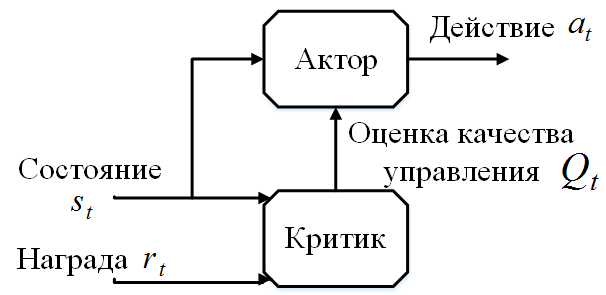
\includegraphics [scale=0.7] {ac}
	\caption{Структурная схема Актор-Критик метода} 
	\label{img:ac}  
\end{figure}

\subsection{Анализ алгоритмов обучения} \label{subsect1_6_7}

\section{Основные выводы по главе 1} \label{sect1_7}
